% This file was created by matplotlib2tikz v0.7.4.
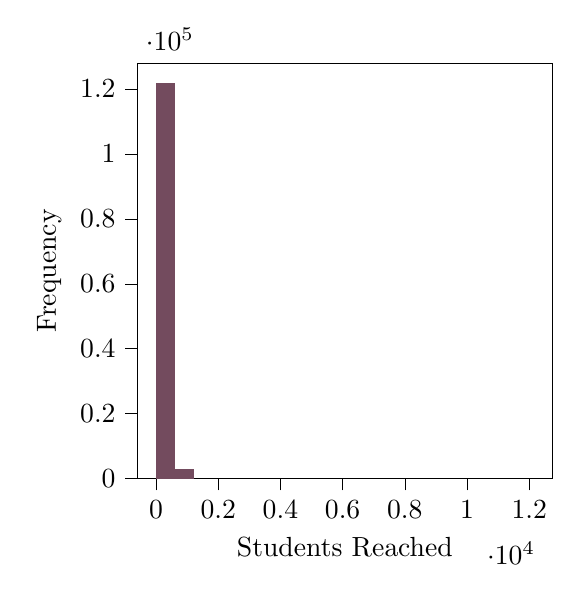
\begin{tikzpicture}

%\definecolor{color0}{rgb}{0.0431372549019608,0.192156862745098,0.258823529411765}
\definecolor{color0}{rgb}{0.450980392156863,0.294117647058824,0.368627450980392}
\begin{axis}[
height=2.7in,
tick align=outside,
tick pos=left,
width=2.7in,
x grid style={white!69.01960784313725!black},
xlabel={\opns{Students Reached}},
xmin=-606.1, xmax=12750.1,
xtick style={color=black},
y grid style={white!69.01960784313725!black},
ylabel={\opns{Frequency}},
ymin=0, ymax=127923.6,
ytick style={color=black},
]

\draw[fill=color0,draw opacity=0] (axis cs:1,0) rectangle (axis cs:608.1,121832);
\draw[fill=color0,draw opacity=0] (axis cs:608.1,0) rectangle (axis cs:1215.2,3078);
\draw[fill=color0,draw opacity=0] (axis cs:1215.2,0) rectangle (axis cs:1822.3,3);
\draw[fill=color0,draw opacity=0] (axis cs:1822.3,0) rectangle (axis cs:2429.4,1);
\draw[fill=color0,draw opacity=0] (axis cs:2429.4,0) rectangle (axis cs:3036.5,0);
\draw[fill=color0,draw opacity=0] (axis cs:3036.5,0) rectangle (axis cs:3643.6,0);
\draw[fill=color0,draw opacity=0] (axis cs:3643.6,0) rectangle (axis cs:4250.7,0);
\draw[fill=color0,draw opacity=0] (axis cs:4250.7,0) rectangle (axis cs:4857.8,0);
\draw[fill=color0,draw opacity=0] (axis cs:4857.8,0) rectangle (axis cs:5464.9,0);
\draw[fill=color0,draw opacity=0] (axis cs:5464.9,0) rectangle (axis cs:6072,0);
\draw[fill=color0,draw opacity=0] (axis cs:6072,0) rectangle (axis cs:6679.1,0);
\draw[fill=color0,draw opacity=0] (axis cs:6679.1,0) rectangle (axis cs:7286.2,0);
\draw[fill=color0,draw opacity=0] (axis cs:7286.2,0) rectangle (axis cs:7893.3,1);
\draw[fill=color0,draw opacity=0] (axis cs:7893.3,0) rectangle (axis cs:8500.4,0);
\draw[fill=color0,draw opacity=0] (axis cs:8500.4,0) rectangle (axis cs:9107.5,0);
\draw[fill=color0,draw opacity=0] (axis cs:9107.5,0) rectangle (axis cs:9714.6,1);
\draw[fill=color0,draw opacity=0] (axis cs:9714.6,0) rectangle (axis cs:10321.7,0);
\draw[fill=color0,draw opacity=0] (axis cs:10321.7,0) rectangle (axis cs:10928.8,0);
\draw[fill=color0,draw opacity=0] (axis cs:10928.8,0) rectangle (axis cs:11535.9,0);
\draw[fill=color0,draw opacity=0] (axis cs:11535.9,0) rectangle (axis cs:12143,1);
\end{axis}

\end{tikzpicture}